\section{Kolo "Toure" Kozolski}

\begin{center}
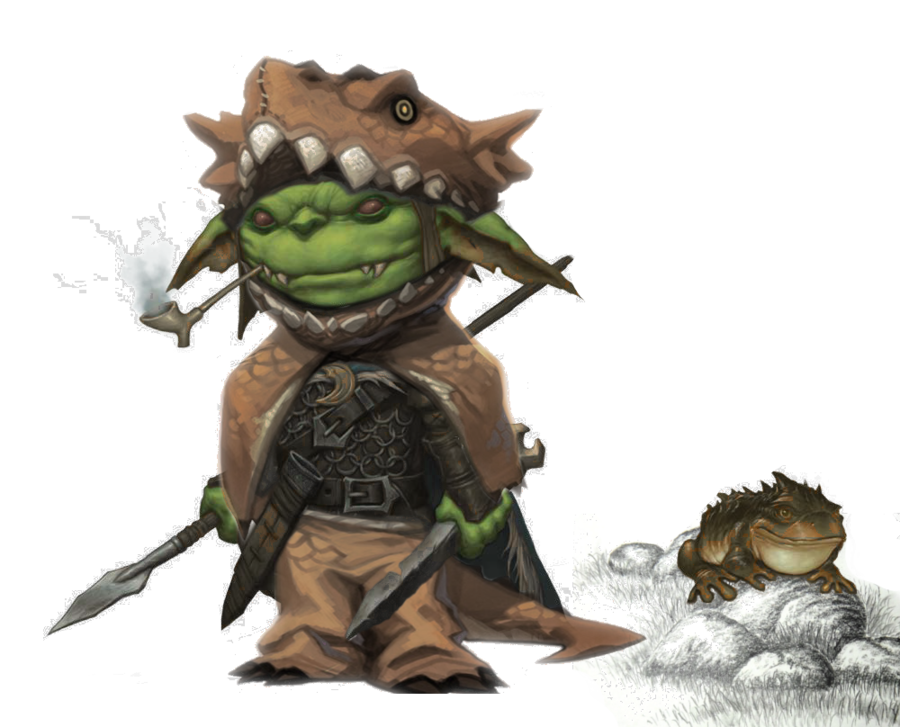
\includegraphics[width=80mm]{./content/img/krokokolo.png}
\begin{figure}[h]
\end{figure}
\end{center}

\subsection*{Details}

\noindent

Race: Goblin\\
Class: Rogue/Ranger\\
Age: 8\\
Status: Dead (ep 68), restored in a construct body (ep 98)

\subsubsection{Background}

Kolo Kozolski was born two minutes after his twin sister Exmerah in the frozen wastelands of ``the North", deep within the territory of the Varg.  Like all Gabrins under Varg rule, the twins were enslaved from birth and spent their early years in bondage.  Where Exme gravitated towards the workshops, Kolo took to the shadows, honing his skills as a thief, scout, and survivalist.

The twins were killed during an audacious escape attempt from their northern stronghold and resurrected by the devil Lazarus in Hell, along with three strangers, to carry out a mission to destroy the Church of the Seven.

\subsubsection{Personality and Traits}

Boisterous, outspoken, and utterly fearless, Kolo was the face and frontman of the goblin duo.  He was a natural leader with a flair for the dramatic, always the first into battle and the last to shut up about it afterwards.

Known for his impossibly fast fingers, Kolo was not to be trusted anywhere near another person's money, property, or indeed pockets.  He relieved Pilcheur of fifteen gold pieces within hours of meeting him and continued a lifelong career of redistributing other people's wealth.

Kolo harboured a burning passion for Gabrin emancipation, though his philosophy differed sharply from his sister's.  Where Exme believed the races could work together, Kolo held that freedom could only be won by the sharp edge of a blade and that the only good human was a dead one.  He was a gifted storyteller, regaling the group with the legendary tale of Grumpy Stanri, the elder goblin emancipator, around the campfire after Otoria's death.

Kolo spoke Tikki Tuck, Goblin, and Low Velterran.

\subsubsection{Relationships}

Kolo's bond with his twin sister Exmerah was the defining relationship of his life.  The two had never spent more than an hour apart before Kolo's descent into darkness, and his final act of lucidity was a scrawled note to her reading simply ``Help me".

He maintained a gleeful antagonism with Pilcheur, whom he referred to exclusively as ``Pilchard" or ``Fishy", taking every opportunity to steal from him and blame others for the consequences.

Kolo shared an unlikely bond with Gary, the ancient stone elemental who became the moral heart of the group.  Gary ultimately sacrificed himself to protect Kolo in the jungles of South Africa, an act of selflessness that Kolo never forgot.

His relationship with Riphard was complex, a mixture of mutual respect, competitive one-upmanship, and deep resentment.  Every slight, every stolen kill, every act of goblin superiority that Kolo visited upon the dwarf accumulated into a debt that Riphard finally collected in the sewers of Hope's Rest.

Kolo formed a bond with Myron through their shared ``turtle power" battle cries and combat tactics during the Masuda campaign, though this friendship did not survive Kolo's corruption.

\subsubsection{Kolo's Story}

Kolo began the campaign as a scrappy, quick-witted rogue who complemented his sister's inventive genius with raw cunning and combat skill.  He was instrumental in retrieving the Stone of Unthala from the ice temple, surviving the Die Hard heist at the Tower of Imota Kan, and founding the Gary Guild in Hope's Rest through sheer force of personality.

During the Masuda campaign, Kolo came into his own as a warrior, adopting the ``turtle power" battle philosophy with Myron and leading devastating charges against orc warbands.  He underwent the Gabrin Coming of Age ritual alongside Exme, emerging physically transformed and stronger than ever.

The turning point came in the Tom'ardy Mountains.  While searching for Excalibrum in the deep mines, Kolo began to hear the whispers of Kalimar, an ancient elder entity with the power to warp flesh.  The corruption took hold gradually, Kolo grew more erratic, more violent, until he murdered his uncle Targon and was turned to stone by Gorgons alongside Myron.

After being destoned, Kolo sacrificed Daisuke to Kalimar in a blood ritual in the depths of the mines, painting Exme's face with the interpreter's blood before vanishing into the darkness.  He resurfaced briefly in Hope's Rest, attempting to recruit Exme and Burnie to Kalimar's cause and orchestrating an ambush involving Burnie's estranged bird-son Trayvon Jr.

When Kolo was finally found in the sewers beneath Hope's Rest, he was barely recognisable, massively mutated with one enormous arm, fungal wings, and a body riddled with Kalimar's corruption.  In the battle that followed, Kolo crushed Delilah Hardstone's skull, killing Riphard's wife.  Exme stopped time with the Puzzle Die to save Delilah's twin babies, but Kolo himself was beyond saving.  Riphard wrapped his whip around Kolo's throat and strangled the life from him, shouting the name of his childhood friend Dagenham as he did so.

Kolo's soul did not pass to Hell.  It was claimed by Kalimar, trapped somewhere beyond even Lazarus's reach.  Exme's last hope was that the return of the gods might free her brother from his eternal prison.

\subsubsection{The Continuation}

Four years after the Spire fell, Kolo's soul remained among tens of thousands trapped inside Kalimar.  When the party tracked the elder god to his lair beneath a giant ice sheet in the far north, Exme saw her chance.  She rigged Kalimar's spawn-egg hatcheries with dynamite and detonated them in the final battle.  Mrs Ball, a sentient sphere of impossibly dense metal, delivered the killing blow, punching clean through the Elder God of Creation.

But the battle had cost everything.  Myron lay dead, stabbed through the chest.  Exme, battered and broken, held the Puzzle Die of Ruh'Breks and its single Wish function, the only wish in existence, with a ten-thousand-year cooldown.  She could save Kolo or she could save Myron.  She chose both.  She wished to give up her own life to restore her brother and heal the gnome she loved.  The wish was accepted, and the price was absolute: Exmerah was erased from all reality, never to be resurrected, never to reach any afterlife.

Kolo woke in a constructed body, mechanical and cold, unable to eat or taste.  The others called him ``Mr Robot''.  His twin sister was gone in a way that even the gods could not undo.  Beside him he found her last gift: a mechanical bow with a cabled power pack, built with the same inventive genius that had produced STANRI and C.E.D.R.I.C.

Standing on the deck of the airship, Kolo addressed the survivors.  ``She changed everything she touched,'' he said.  ``This boat, your leg and eye, and you Myron, she changed you.  I never loved any of you, not like I did her.  But if you are the only parts of her that remain, then you are the only parts I can keep alive.''

Kolo fought on.  He joined the party as they tracked west to Jecede, watched Erin die aboard a githyanki Nautiloid, saw Burnie torn apart by the elder brain, and rode the maiden-voyage steam railway to Hope's Rest with the remnant of the group.  He debuted Exme's mechanical bow in a rooftop fight against Inquisitors on the train, and shot at a telepathic sewer octopod called Badunkadonk beneath Hope's Rest, nearly undoing Gem's careful diplomacy with the creature.  He joined the heist of the deserted Black Rock bank and descended into the vault to claim the Armoury of Sin, the divine gear the god Sinn wore when he last fought Canalon.

The goblin who had been dead, corrupted, and trapped inside an elder god for four years walked out of that vault carrying a god's armour, heading to fight another one.  Exme would have been proud.

\begin{center}
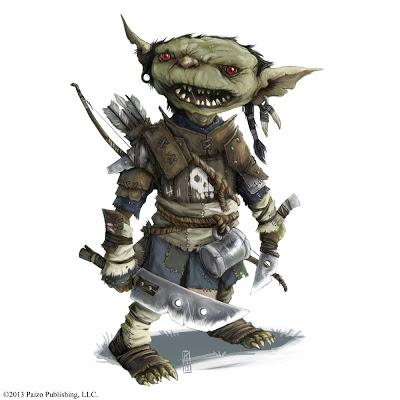
\includegraphics[width=80mm]{./content/img/kolo.jpg}
\begin{figure}[h]
\end{figure}
\end{center}

\begin{DndSidebar}{Kolo's Tale}
Following Otoria's death, Kolo told the group the story of Grumpy Stanri, a legendary goblin cleric and emancipator who assembled a crack team of Gabrins, the deadly archer Tan'lata, the rage-filled Kri'igo, and the useless Dev'lada with his greasy weasel, on a quest to free goblin-kind.  The tale of their voyage across treacherous seas and through the ruins of Thundertree is recorded in Episodes 9b through 9d.
\end{DndSidebar}

\clearpage
